\subsection{Conditioning input data}
	Working in the time domain, the data is usually transformed to the frequency domain to analyse where the pattern is found more easily. Also, ergardless of the chosen model, we will work in high dimensions which means we need a lot of input data in order to find the pattern. In the case of SVMs, it will be high-dimensional training points $\{\vec x^{(i)}\}_1^m$; in the case of SSMs and HMMs, it will be the high-dimensional observed variables $\{\vec y_t\}_1^T$. We will present two ways to condition the input data, before analysing it using the learning algorithms above, namely frequency-domain analysis and Principal Components Analysis.
	
	\subsubsection{Frequency-domain analysis}
		\paragraph{Discrete Fourier Transform.}
			Discrete Fourier Transform (DFT) is used to transform a finite list of equally spaced samples of a function into the list of coefficients of a finite combination of complex sinusoids \cite{wiki:DFT}. It can be said to convert the sampled function from its original domain to the frequency domain \cite{wiki:DFT}. The DFT, $\mathcal{F}$, can be defined to transform $\vec x = \{x_1, x_2, \dotsc, x_{N}\}$ to $\vec X = \{X_1, X_2, \dotsc, X_{N}\}$ as
			\begin{equation}
				X_k = \sum_{n = 1}^{N} x_n \exp{(-i2\pi k n / N)}, 1 \leq k \leq N
			\end{equation}
			and can be performed using the Fast Fourier Transform (FFT) algorithm.

		\paragraph{Power Spectral Density.}
			It is common to take the Power Spectral Density (PSD) instead of the DFT in order to remove the imaginary components in the frequency domain. The PSD of a continuous signal $x(t)$ can be defined as
			\begin{equation}
				S_{xx}(f) = \lim_{T \to \infty} \frac{1}{T} \left| X(f) \right|^2
			\end{equation}
			where $X(f)$ is the Fourier transform ($\mathcal{FT}$) of $x(t)$ in the interval $-T / 2 < t < T / 2$ \cite{hlt}. It can be shown that in the discrete case where $\vec x = \{x_1, x_2, \dotsc, x_{N}\}$, the PSD is obtained by
			\begin{align}
				S_{xx}(k) 	&= \lim_{T \to \infty} \frac{(\Delta t)^2}{T} |X_k|^2\\
							&\approx \frac{(\Delta t)^2}{T} |X_k|^2
			\end{align}
			where $T$ is the actual recording time, $N$ is number of samples and $1/\Delta t$ is the sampling frequency (note that $T = N(\Delta t)$) \cite{wiki:PSD}.

		\paragraph{Spectrograms.}
			To create a spectrogram of a signal $\vec x = \{x_1, x_2, \dotsc, x_N\} = \{x(\Delta t), x(2\Delta t), \dotsc, x(N\Delta t)\}$, we must choose a window size $T_\text{window}$ and an offset $T_\text{offset}$. Then, we keep shifting the window by $T_\text{offset}$ and each time, we transform and store the window's content (in time domain) to the frequency domain using the DFT. This way, we will have a frequency domain data of the size $T_\text{window}$ every $T_\text{offset}$, which we will call $\vec X_1, \vec X_2, \dotsc, \vec X_\tau$. We usually represent this frequency domain data using colour intensities and plot them as $\tau$ columns of colour intensities with time on the horizontal axis and frequency on the vertical axis. Figure \ref{fig:spec} illustrates the process of creating a spectrogram. However, it is common to find the PSDs instead of the DFTs of the sliding windows (the principle stays the same). Hence we will refer to the process of creating the spectrogram with PSDs (instead of DFTs) of the sliding windows as \emph{freqency analysis of the signal}.
			\begin{figure}[ht]
				\centering
					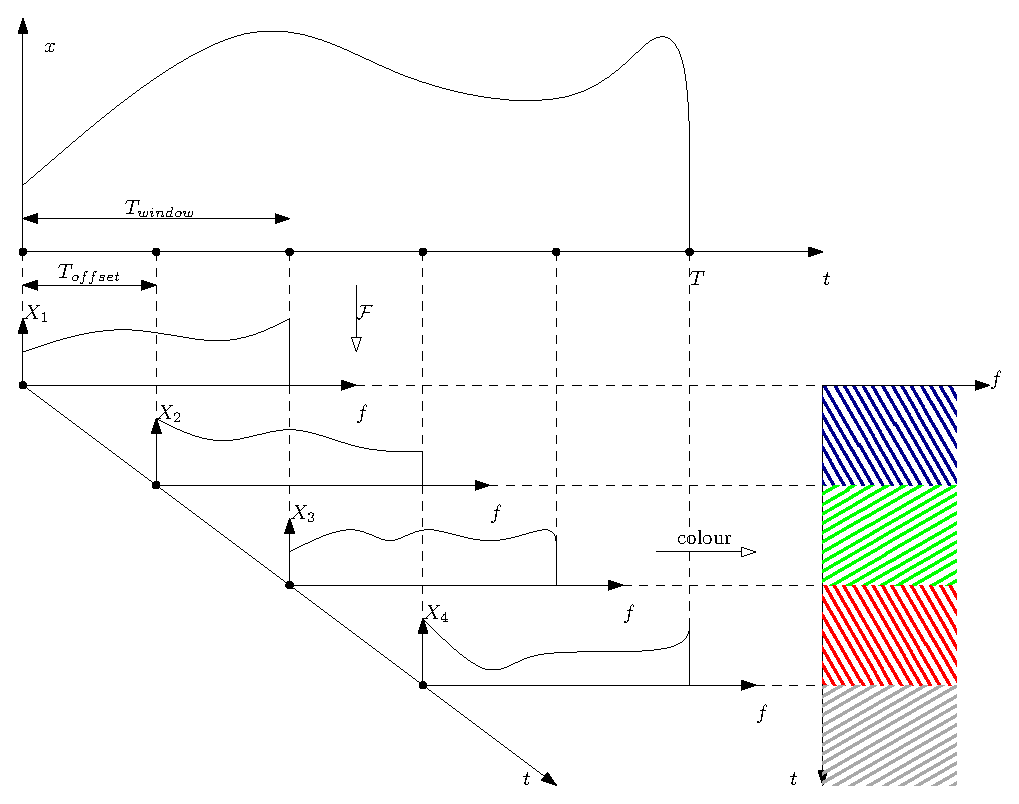
\includegraphics{drawings/spec.eps}
				\caption{The process of creating a spectrogram.}
				\label{fig:spec}
			\end{figure}

	\subsubsection{Principal Components Analysis}
		Here we present the theory for Principal Components Analysis (PCA) based on Andrew Ng's lecture notes \cite{ng13} and Kevin Murphy's book \cite{mlBook}. The objective is to take $m$ $n$-dimensional input data points $\{\vec x^{(i)} \in \mathbb{R}^n\}_1^m$ and transform them into $m$ $k$-dimensional data points ($k<n$) $\{\vec y^{(i)} \in \mathbb{R}^m\}_1^m$, where $\vec y^{(i)}$'s are projections of $\vec x^{(i)}$'s onto $k$ orthonormal basis vectors $\{\vec u_i\}_1^k$ while ``preserving the most variance''. We assume that over all $m$ points, their $\text{mean}\left[\{x^{(i)}_j\}_{i = 1}^m\right] = 0$ and their $\text{var}\left[\{x^{(i)}_j\}_{i = 1}^m\right] = 1$ for all features of the input points $1 \leq j \leq n$. We normalise the data first if this is not the case. For $n = 2$, $k = 1$, Figure \ref{fig:pca} shows the projections to the new axis.
		\begin{figure}[ht]
			\centering
				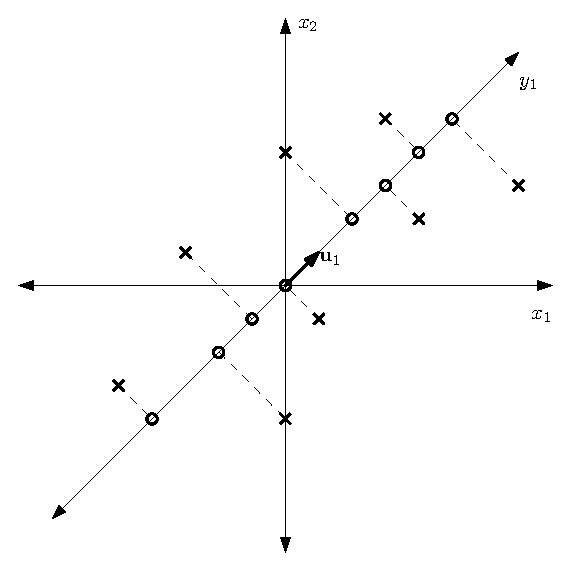
\includegraphics{drawings/pca.eps}
			\caption{Illustration of PCA.}
			\label{fig:pca}
		\end{figure}

		We can see that the transformed points can be expressed as
		\begin{equation}
		 	\vec y^{(i)} =
		 		\begin{bmatrix}
		 			\vec u_1^T \vec x^{(i)} \\
		 			\vec u_2^T \vec x^{(i)} \\
		 			\vdots \\
		 			\vec u_k^T \vec x^{(i)} \\
		 		\end{bmatrix}
		 		, 1 \leq i \leq m
			\label{eqn:pca}
		\end{equation}
		
		It can be shown that in order to maximise $\sum_{i = 1}^m \left\| \vec y^{(i)} \right\|^2$, conditioned on orthonormality of the bases, we must choose normalised eigenvectors corresponding to the $k$ largest eigenvalues of the variance matrix $\vec \Sigma = \frac{1}{m} \sum_{i = 1}^m \vec x^{(i)} {\vec x^{(i)}}^T$ as the bases. These bases are also called the \emph{principal components}. The eigenvalues are proportional to the actual variances of data in the new bases. Hence, we can compare the relative ``importance'' of the bases and use this fact to decide how many principal components to use.